\documentclass[11pt]{article}
\usepackage[margin=1in]{geometry}
\usepackage{amsmath,amssymb}
\usepackage{graphicx}
\usepackage{booktabs}
\usepackage{hyperref}
\usepackage{natbib}
\usepackage{doi}
\usepackage{subcaption}
\renewcommand{\topfraction}{0.9}\renewcommand{\textfraction}{0.08}\renewcommand{\floatpagefraction}{0.7}\setcounter{topnumber}{3}
\hypersetup{colorlinks=true,linkcolor=blue,citecolor=blue,urlcolor=blue}
% Generated by scripts/make_figures.py. Do not edit.
\newcommand{\NumParams}{81.9}
\newcommand{\NumParamsExact}{81,912,576}
\newcommand{\NumTensors}{76}
\newcommand{\WeightFileMB}{163.8}
\newcommand{\WeightFpThirtyTwoMB}{327.7}
\newcommand{\VocabSize}{50,257}
\newcommand{\LoadMsSim}{177}
\newcommand{\ExpandMsSim}{78}
\newcommand{\TokLoadMsSim}{98}
\newcommand{\LatOneSim}{89}
\newcommand{\LatEightSim}{85}
\newcommand{\LatShortMinSim}{83}
\newcommand{\LatShortMaxSim}{93}
\newcommand{\LatSixteenSim}{94}
\newcommand{\LatFortyEightSim}{132}
\newcommand{\LatFortyEightPninetySim}{137}
\newcommand{\FootprintDeltaMBSim}{339}
\newcommand{\FootprintPeakMBSim}{339}
\newcommand{\EncodeUsSim}{38}
\newcommand{\RepeatsSim}{20}
\newcommand{\ThermalSim}{nominal}
\newcommand{\DeviceLabelSim}{iOS Simulator (iPhone19,2) on Apple M1 Max}
\newcommand{\OSVersionSim}{Version 27.0 (Build 24A434)}
\newcommand{\DeviceRows}{Simulator / M1 Max & 177 & 89.3 & 85.1 & 94.2 & 118.0 & 132.2 & 339 \\}
\newcommand{\NumDevices}{1}
\newcommand{\AgreePrompts}{3}
\newcommand{\AgreeTopTenExact}{3}
\newcommand{\AgreeLensExact}{18/18}
\newcommand{\AgreeMaxProbErr}{2.0\times10^{-6}}
\newcommand{\AgreeMaxNormRel}{3.5\times10^{-7}}
\newcommand{\AgreeMaxAttnErr}{6.5\times10^{-7}}
\newcommand{\FidPrompts}{30}
\newcommand{\FidTopOne}{30}
\newcommand{\FidTopThree}{30}
\newcommand{\FidKLMeanBits}{3.7}
\newcommand{\FidKLMaxBits}{7.9}
\newcommand{\FidMaxDp}{0.18}
\newcommand{\FidWeightErrMedian}{2.1}
\newcommand{\FidWeightErrMax}{3.1}
\newcommand{\FidWorstPrompt}{In 1969, astronauts first landed on the}
\newcommand{\FidWorstToken}{moon}
\newcommand{\FidWorstPthirtytwo}{36.02}
\newcommand{\FidWorstPsixteen}{35.84}
\newcommand{\CostRows}{1 & 42 & 0.0 & 270 & 313 & 86\% \\
8 & 340 & 0.6 & 270 & 611 & 44\% \\
16 & 679 & 2.4 & 270 & 952 & 28\% \\
32 & 1359 & 9.4 & 270 & 1639 & 16\% \\
48 & 2038 & 21.2 & 270 & 2330 & 12\% \\}
\newcommand{\LensShareOne}{86}
\newcommand{\LensShareFortyEight}{12}
\newcommand{\UnembedMMAC}{38.6}
\newcommand{\UnembedTotalMMAC}{270}
\newcommand{\BlockMMACPerToken}{42.5}
\newcommand{\GflopsFortyEightSim}{35}


\title{Orch Neural Network:\\A Fully Traced GPT-2 Running Natively on iPhone\\to Show How Next-Word Prediction Works}
\author{Wonmo (John) Seong\\ \small Chief Scientific Officer, Orchestr Aerospace Inc.\\ \small \href{mailto:john@orchestrsim.com}{john@orchestrsim.com}}
\date{October 2026}

\begin{document}
\maketitle

\begin{abstract}
Most interactive explanations of transformer language models run in a browser against a server or a JavaScript port, and most on-device inference engines optimise away exactly the intermediate values an explanation needs. We describe Orch Neural Network, an iOS app that runs DistilGPT2 (\NumParams M parameters) from scratch in Swift on Apple's Accelerate framework and records everything the forward pass computes: the tokens, the embedding vector, all $12\times6$ attention matrices, the 3{,}072 MLP activations of every layer, a logit-lens prediction after every layer, the final distribution over \VocabSize\ tokens, and every one of the \NumTensors\ weight tensors, which can be browsed as heatmaps. The app frames the model as the thing behind a phone keyboard's three word suggestions, and a guided walkthrough explains one forward pass on the user's own text. Weights are stored in a 64-byte-aligned float16 container (\WeightFileMB~MB) and expanded to float32 at load. We verify the implementation against an independent NumPy forward pass on the same weights (top-10 ranking identical on all test prompts; probabilities agree to $\AgreeMaxProbErr$) and measure the cost of float16 storage against the original float32 release (top-1 and top-3 agreement on \FidTopOne/\FidPrompts\ prompts; mean KL of $\FidKLMeanBits\times10^{-5}$ bits). A traced pass takes \LatShortMinSim--\LatFortyEightSim~ms for 1--48 tokens in the iOS Simulator on an M1 Max, and an analytic cost model shows that for short inputs the logit lens, not the transformer, dominates: at one token the seven unembedding products are \LensShareOne\% of the arithmetic. The deliberate omissions (no KV cache, no fused kernels, full recomputation on every keystroke) are what make every value inspectable. Code, weights converter, benchmark harness and this manuscript are open.
\end{abstract}

\section{Introduction}
A phone keyboard's suggestion bar is the most widely used language-model interface in existence, and almost nobody who uses it knows that the three words it offers are the top of a probability distribution produced by a neural network \citep{hard2018}. The same mechanism, scaled up, is a chatbot. Interactive visualisations of transformers \citep{vig2019,hoover2020,cho2024,bycroft2023} have made the mechanism far more approachable, but they run in a browser, usually against a server or a JavaScript re-implementation, and they stop at the activations: the weights that produce them are not shown, because there are too many of them.

We wanted to put the whole thing on the device people actually type on, and to show all of it: every intermediate value of a real GPT-2 forward pass, and every weight matrix, on a phone, offline, with the user's own sentence as input. The constraints of that setting are instructive. A phone has a few gigabytes of memory and a thermal budget; a model that can be fully traced on every keystroke must be small; and the engine must be written so that nothing is optimised away. The result is a from-scratch Swift implementation of DistilGPT2 \citep{sanh2019,radford2019} on Accelerate that recomputes the full sequence on every input change and keeps every activation, together with a compact weight container and a four-screen interface built around a QuickType-style suggestion bar.

This paper is a systems and verification report, not a learning study. We describe the implementation (Sec.~\ref{sec:system}), show that it agrees with an independent reference and that float16 storage costs essentially nothing in prediction quality (Sec.~\ref{sec:verify}), measure load time, latency and memory and decompose the cost analytically (Sec.~\ref{sec:perf}), and discuss what a phone can and cannot show (Sec.~\ref{sec:discussion}). Every number in the text is written by the analysis scripts into a macro file that this manuscript includes, so the prose cannot drift from the measurements.

\section{Related work}
\paragraph{Attention and activation visualisers.} BertViz \citep{vig2019} introduced the now-standard head, model and neuron views of attention. exBERT \citep{hoover2020} added corpus search over hidden representations. Transformer Explainer \citep{cho2024} is the closest prior system to ours: a browser-based GPT-2 (small) with live attention, MLP and output-probability views driven by user text. LLM Visualization \citep{bycroft2023} walks through nano-GPT in 3D. Our contribution relative to these is not the idea of visualising a transformer but where and how completely it is done: native, offline, on the user's phone, with every weight tensor browsable and with a verified from-scratch engine rather than a port.

\paragraph{Interpretability tooling.} The logit lens \citep{nostalgebraist2020} and its calibrated successor the tuned lens \citep{belrose2023} read a prediction from the residual stream after each layer; we use the plain lens because it needs no extra parameters. TransformerLens \citep{nanda2022} and the circuits programme \citep{elhage2021} provide hooked models for research; our engine is in effect a fully hooked model with the hooks always on. \citet{geva2021} motivate showing MLP activations as key--value memories.

\paragraph{On-device inference.} llama.cpp \citep{gerganov2023}, MLX \citep{hannun2023} and Core ML target throughput and use KV caches, quantisation and fused kernels. Apple's own on-device foundation model \citep{apple2024} is about forty times larger than ours and is not inspectable. We go the other way: the engine is deliberately unoptimised so that it is transparent, and we quantify what that costs.

\section{System}\label{sec:system}
\subsection{Model and weight container}
The model is DistilGPT2 \citep{sanh2019}: 6 layers, 12 heads, $d=768$, a 4$\times$ MLP, GELU \citep{hendrycks2016} in its tanh form, learned positional embeddings and a tied unembedding over the \VocabSize-token GPT-2 byte-level BPE vocabulary \citep{sennrich2016,radford2019}; \NumParamsExact\ parameters in \NumTensors\ tensors. A Python script converts the Hugging Face safetensors release to our own container, \texttt{TSW1}: a 4-byte magic, a little-endian length, a JSON header holding the model configuration and a tensor table (name, shape, dtype, offset, size), zero padding to a 64-byte boundary, then the tensors as raw little-endian float16 at 64-byte-aligned offsets, in Hugging Face's Conv1D $[\mathrm{in},\mathrm{out}]$ layout so that no transposes are needed. The file is \WeightFileMB~MB and is memory-mapped; the header is parsed in under a millisecond. Storing float16 halves the download and lets the Weights screen sample any matrix on a coarse grid directly from the mapping without materialising it (Sec.~\ref{sec:ui}). At load, every tensor is expanded once to float32 with vImage, because Accelerate's BLAS is single precision; the cost of this choice is measured in Sec.~\ref{sec:perf}.

\subsection{A forward pass that keeps everything}
The engine is a single Swift class of under 300 lines. For input ids $t_1\ldots t_T$ it forms $x = W_E[t] + W_P[1{:}T]$ and then, per layer, LayerNorm, a fused QKV projection via \texttt{cblas\_sgemm}, per-head $QK^\top/\sqrt{d_h}$ and causal softmax, $AV$, the output projection and residual add, then LayerNorm, the two MLP matmuls with GELU between, and the second residual add. After each layer it applies the final LayerNorm to the last position and multiplies by $W_E^\top$ to obtain the logit-lens distribution. The trace returned to the interface contains the token ids and strings, the last token's embedding norm and a 64-value preview, and for every layer the $12$ attention matrices ($T\times T$ each), the top-5 logit-lens tokens, the residual norm, all 3{,}072 GELU outputs for the last position and the fraction above zero; finally the top-$k$ of the output distribution and the elapsed time.

Three ordinary optimisations are absent on purpose. There is no KV cache: the whole sequence is recomputed on every keystroke so that attention over all positions is available for display and so that the code is the textbook algorithm. There is no fusion of LayerNorm, bias or activation into the matmuls. And the softmax is written out in a loop with the causal mask applied explicitly. Inputs are capped at 48 tokens; longer text keeps its suffix. Trailing whitespace is stripped before tokenising because a keyboard predicts the next \emph{word}, and GPT-2 would otherwise treat the lone space as a token and predict word fragments.

\subsection{Tokeniser}
GPT-2's byte-level BPE is re-implemented in Swift from \texttt{vocab.json} and \texttt{merges.txt}: the pre-tokenisation regular expression, the byte-to-unicode table, rank-ordered merging with a per-word cache, and exact round-trip decoding. Encoding a 61-token sentence takes \EncodeUsSim~$\mu$s.

\subsection{Interface}\label{sec:ui}
\begin{figure}[t]\centering
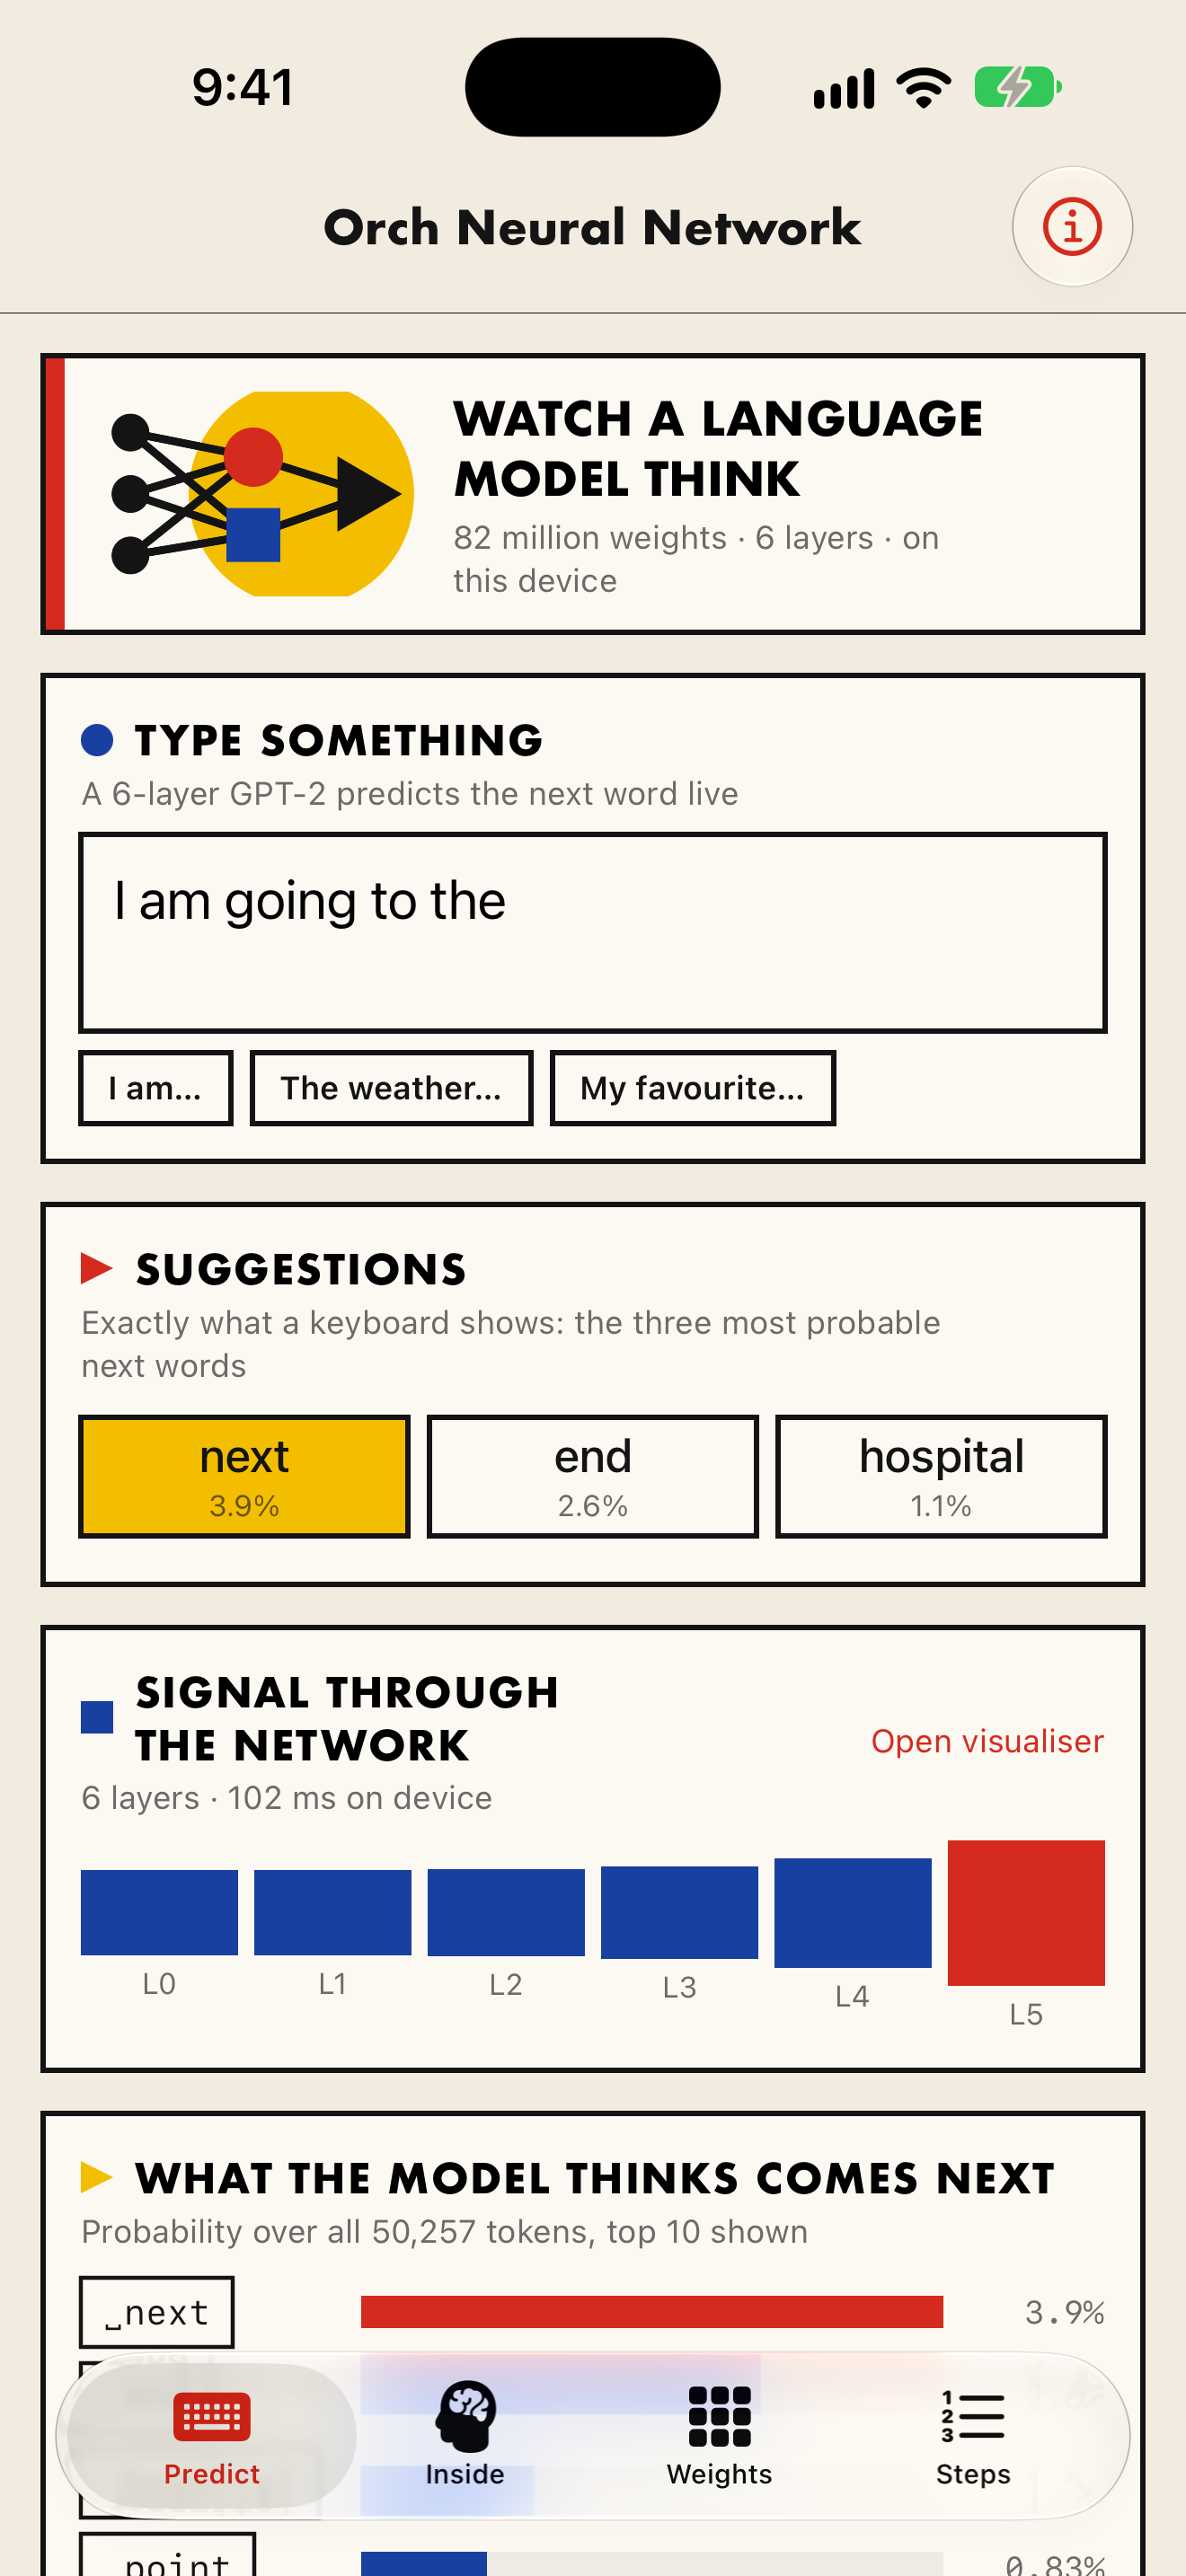
\includegraphics[width=0.235\textwidth]{../screenshots/iphone-6.9-01-predict.png}\hfill
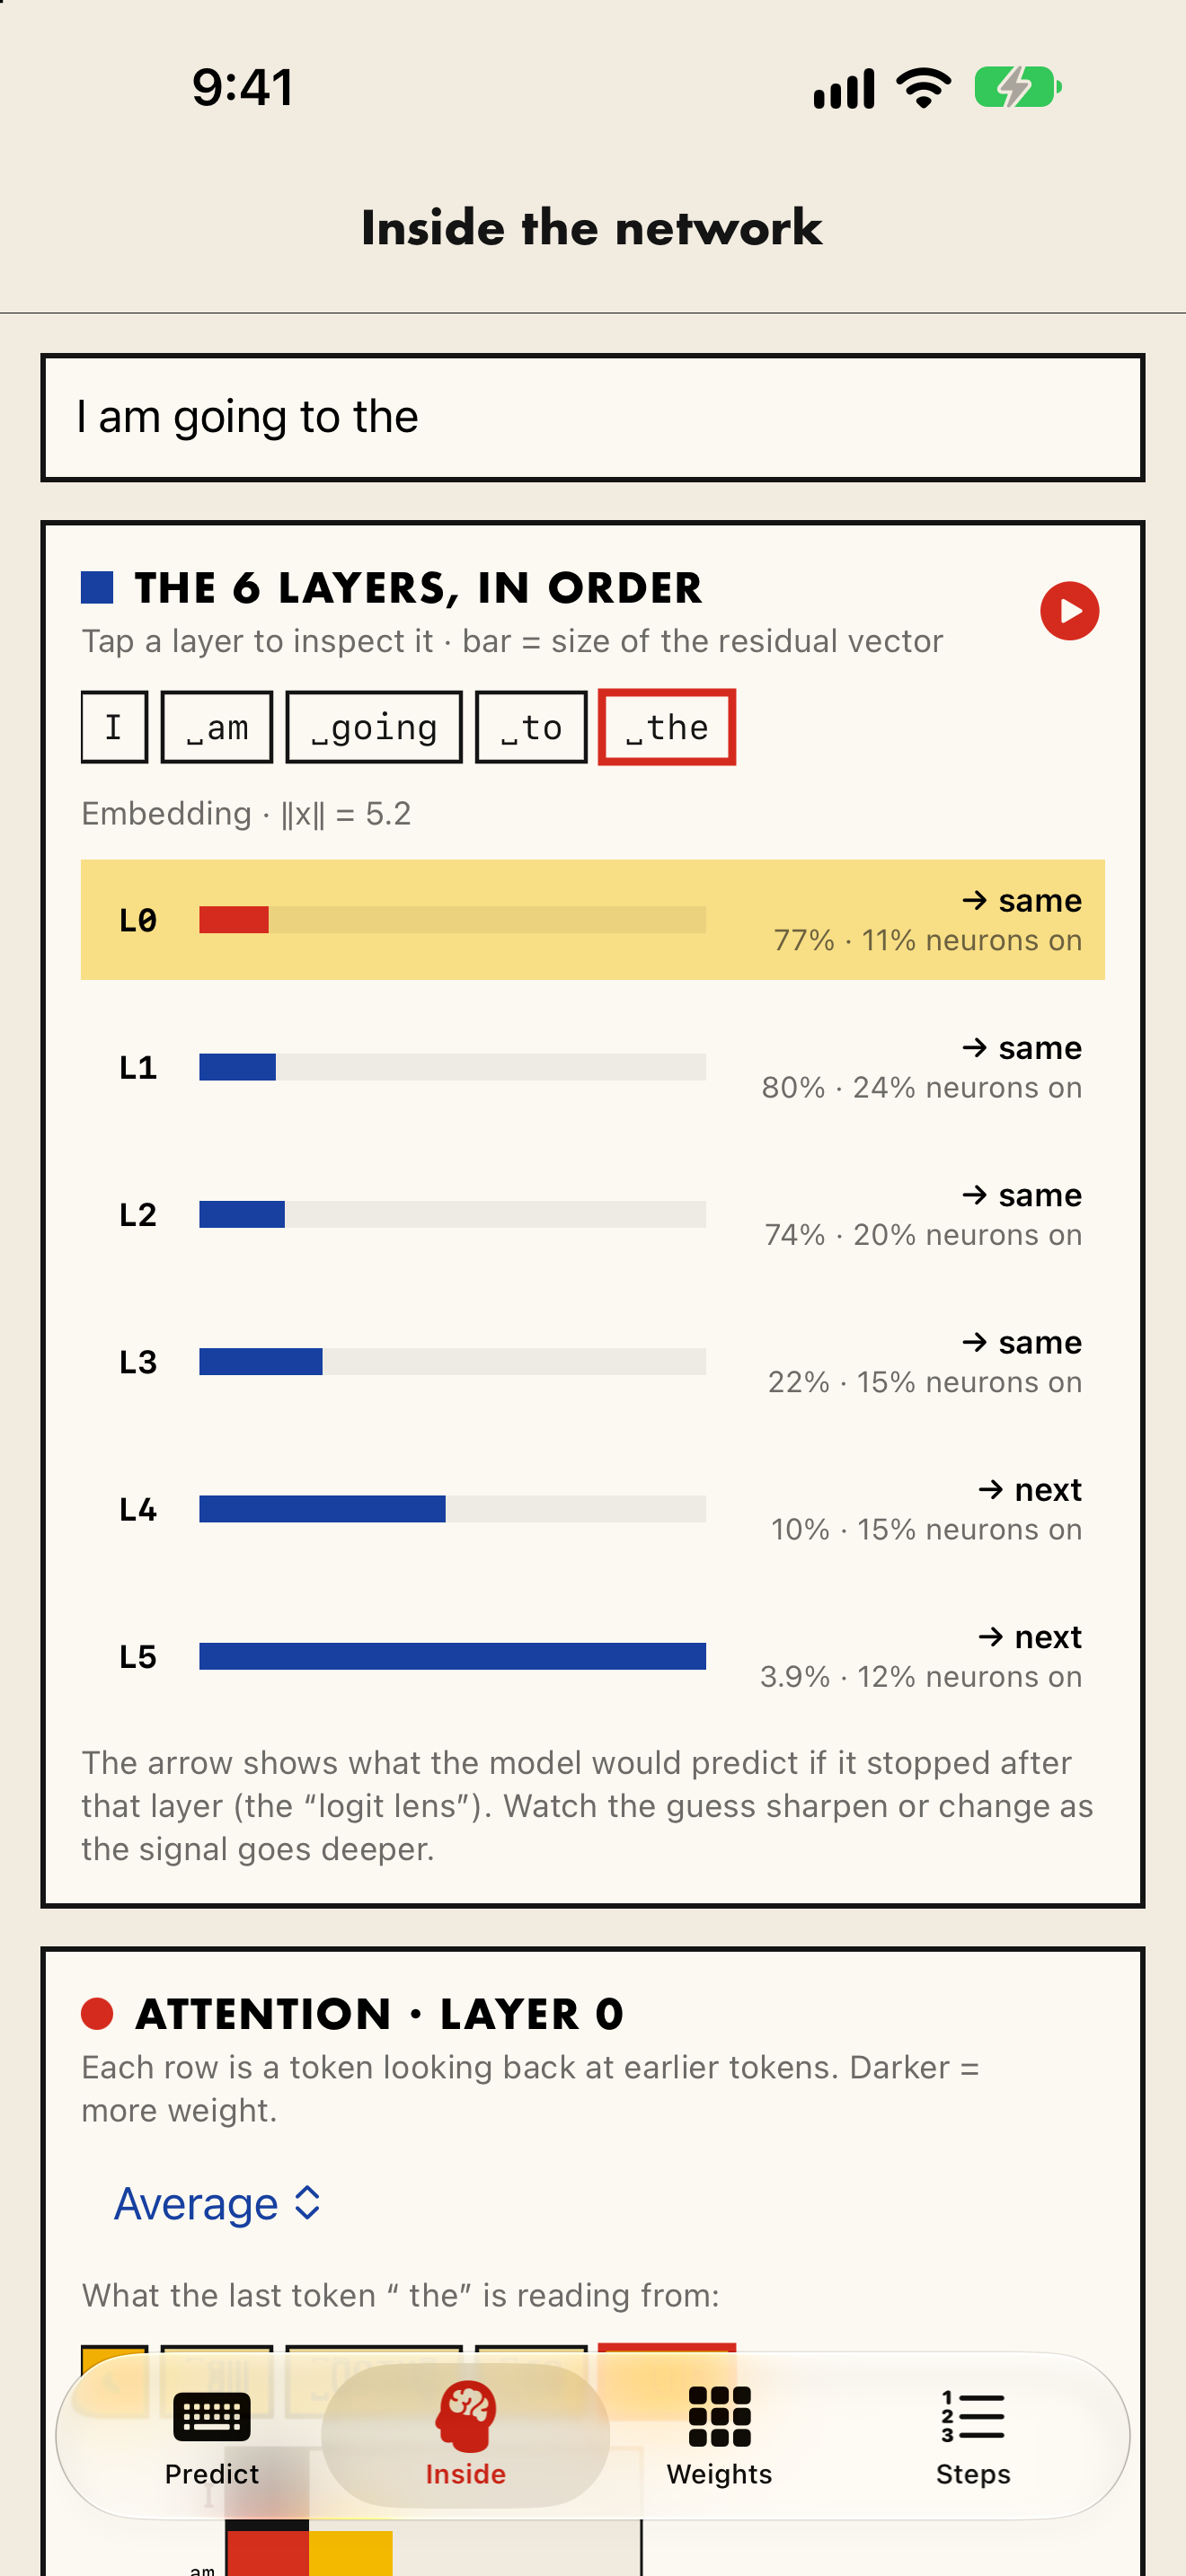
\includegraphics[width=0.235\textwidth]{../screenshots/iphone-6.9-02-inside.png}\hfill
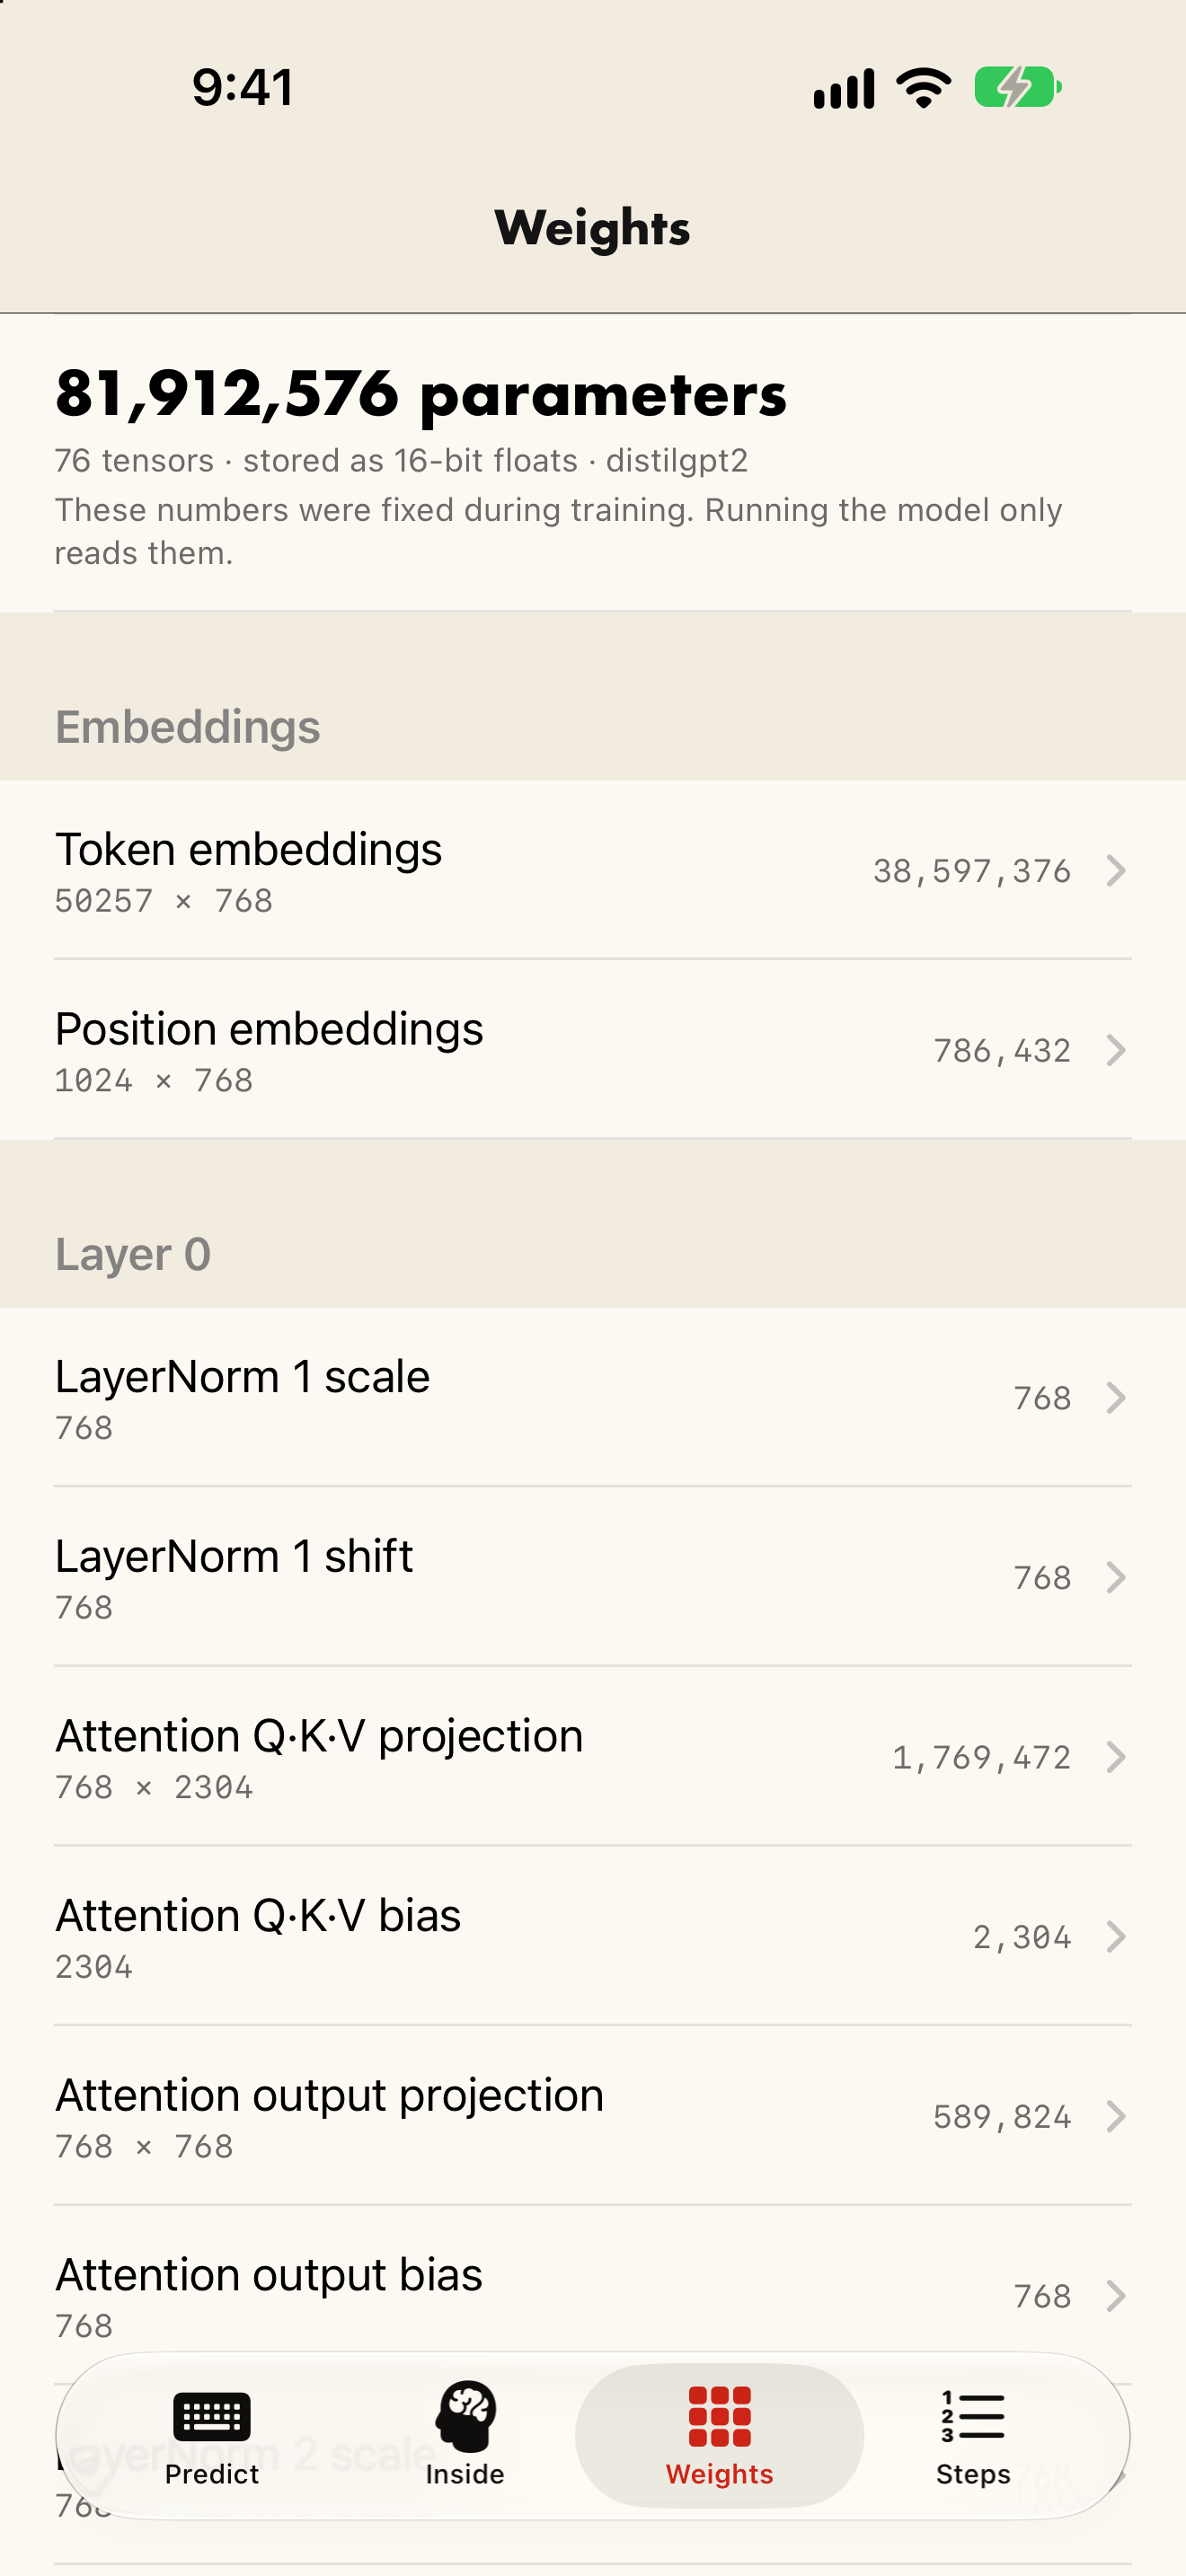
\includegraphics[width=0.235\textwidth]{../screenshots/iphone-6.9-03-weights.png}\hfill
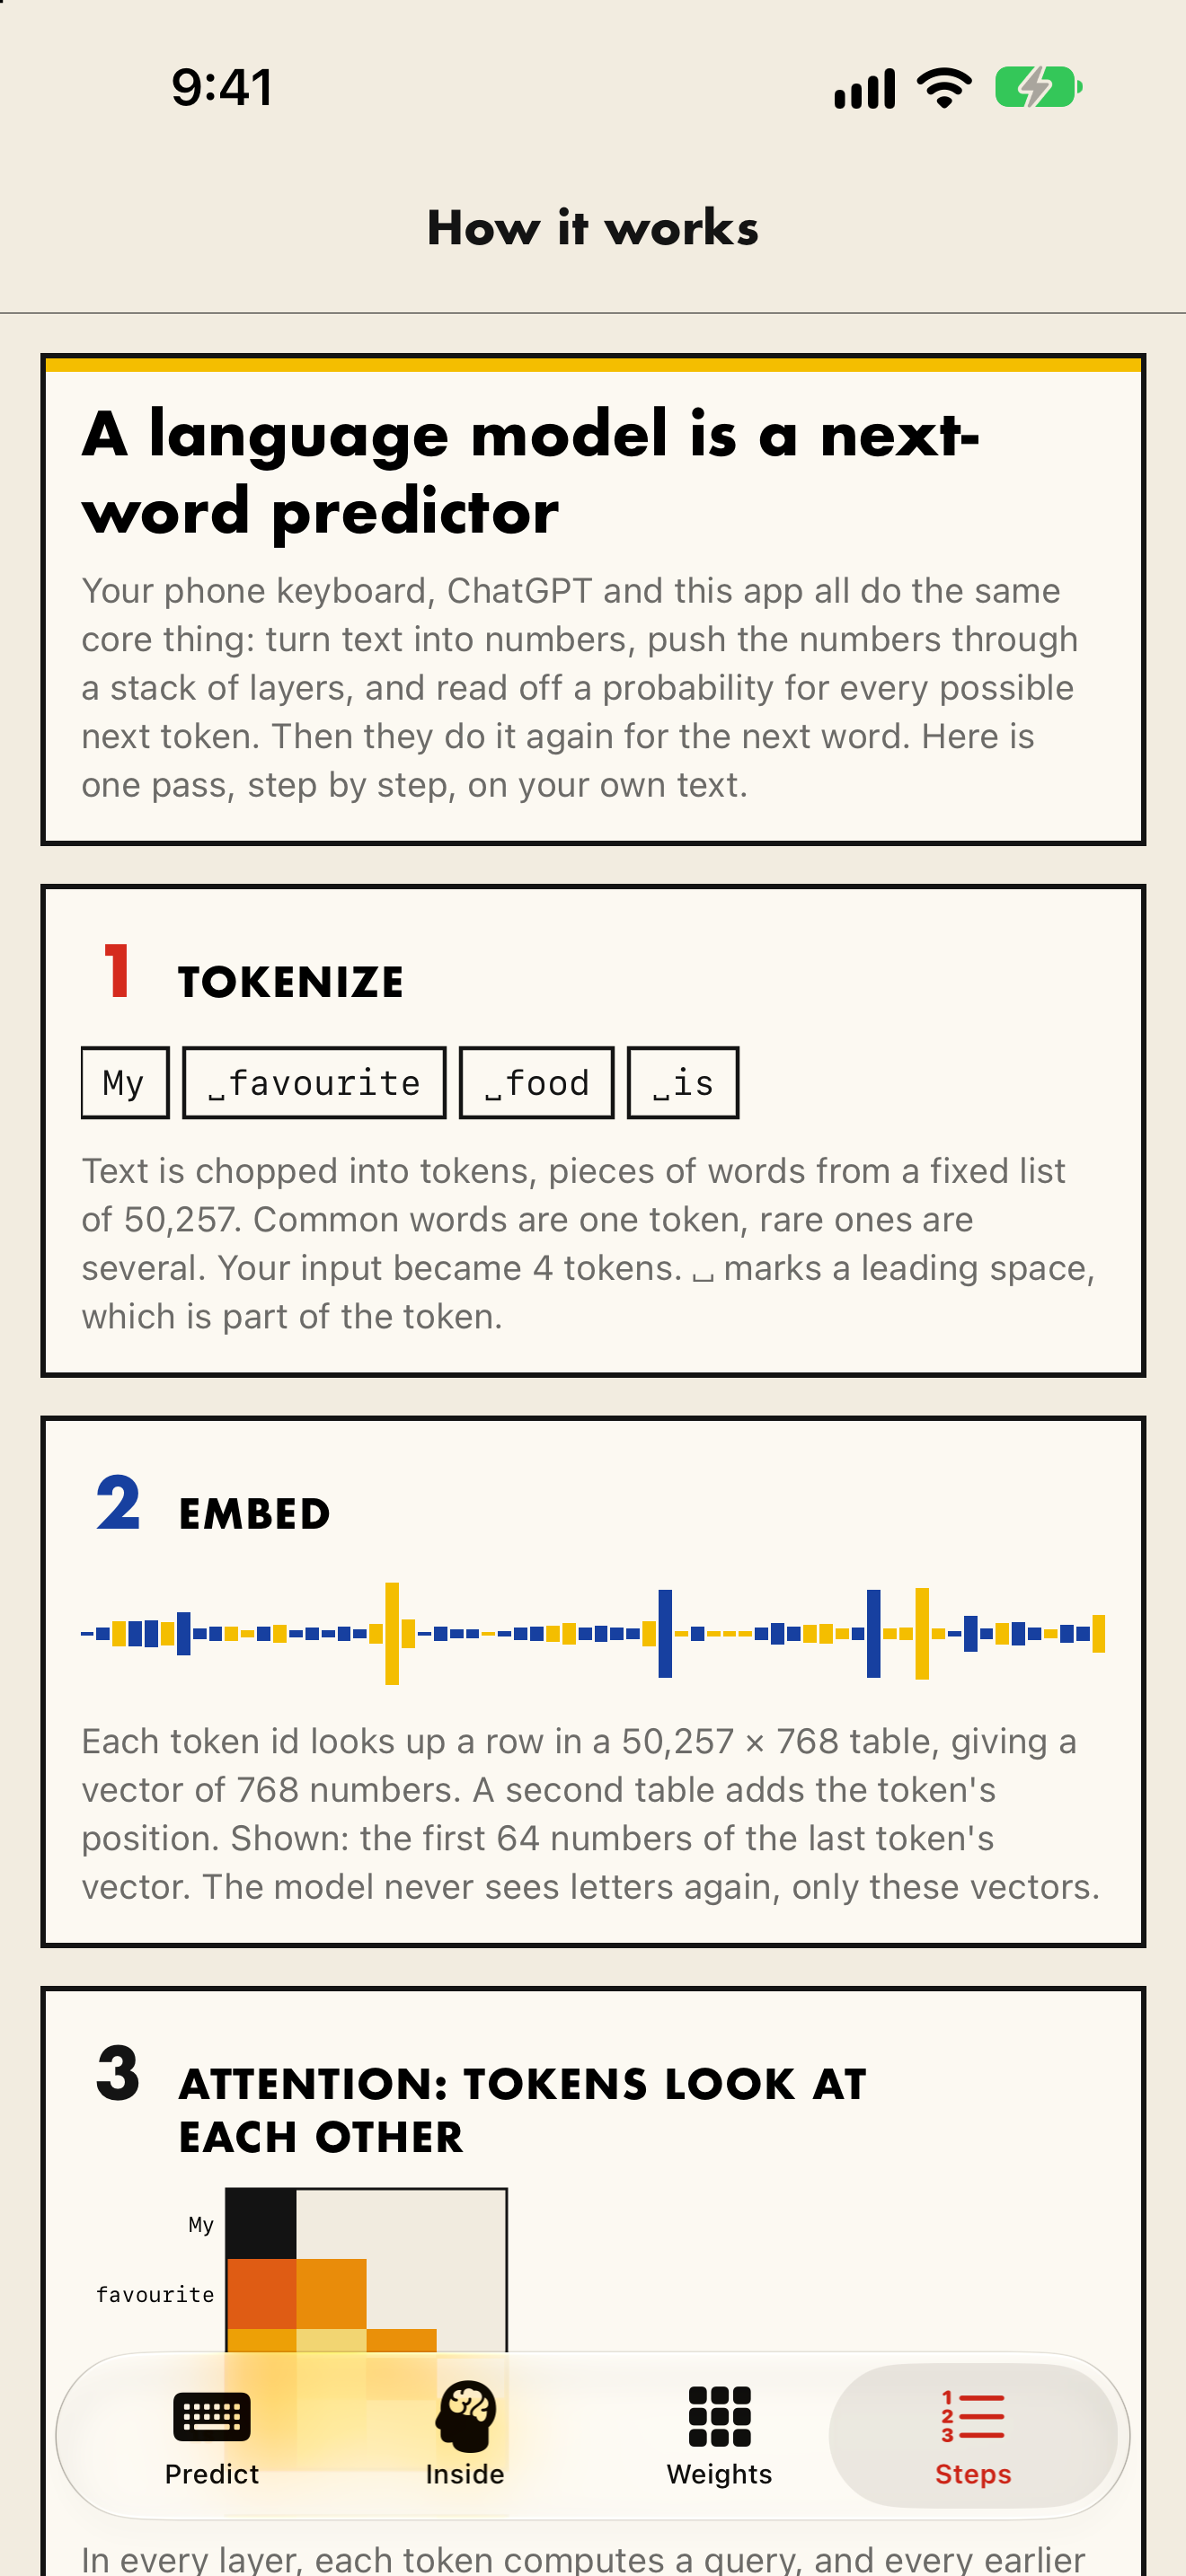
\includegraphics[width=0.235\textwidth]{../screenshots/iphone-6.9-04-learn.png}
\caption{The four screens on iPhone. Left to right: Predict (suggestion bar, layer pulse, output distribution, tokens); Inside (layer stack with logit lens and residual norms, attention heatmap with head picker, MLP neuron grid); Weights (every tensor, grouped by layer, each opening as a heatmap); Learn (the six-step walkthrough on the user's text).}
\label{fig:screens}\end{figure}
Figure~\ref{fig:screens} shows the four tabs. \textbf{Predict} is the hook: a text field, a three-slot suggestion bar that behaves like the system keyboard's, a six-bar pulse that lights in sequence when a pass completes, and the top-10 output distribution with the tokenisation below. Suggestions are derived from the raw distribution the way a keyboard would do it: candidates must be alphabetic (apostrophes allowed), a token with a leading space starts a new word while one without continues the word being typed, duplicates are merged case-insensitively, a short blocklist removes slurs, and the first three survivors are shown with their probabilities. Tapping one inserts it and reruns the model, which is exactly the loop a keyboard performs. \textbf{Inside} is the visualiser: the six layers as a stack, each with the residual norm as a bar and the logit-lens top token with its probability and the fraction of MLP neurons active, animated as a replay through the layers; an attention heatmap for the selected layer with a picker for the head-average or any of the twelve heads, and a token strip showing what the last token attends to; and the 3{,}072 GELU outputs as a $32\times96$ grid. \textbf{Weights} lists all \NumTensors\ tensors grouped by layer with human names (``Attention Q$\cdot$K$\cdot$V projection'', 768~$\times$~2304) and opens any of them as a heatmap sampled from the float16 mapping, including the $50{,}257\times768$ token embedding. \textbf{Learn} is a six-step explanation (tokenise, embed, attention, MLP, six layers and the logit lens, read off probabilities) in which every illustration is computed from the user's current text, and it closes with the reason a network cannot be drawn in full: this small model has \NumParamsExact\ weights and a 4K display has about eight million pixels.

The app has no network access, no accounts and no analytics; it requires iOS~17 and runs on iPhone and iPad.

\section{Verification}\label{sec:verify}
\subsection{Agreement with an independent reference}
A separate NumPy implementation (its own tokeniser and forward pass, sharing only the \texttt{TSW1} reader) generates a reference file for \AgreePrompts\ prompts: token ids, top-10 output tokens and probabilities, per-layer residual norms, per-layer logit-lens tokens, and two full attention rows (layer~0 head~0 and layer~5 head~11). A unit test compares the Swift engine against it and runs in continuous integration. The results in Table~\ref{tab:agree} come from the benchmark harness rather than the test so that they carry full precision. Tokenisation is identical, the top-10 ranking is identical on \AgreeTopTenExact/\AgreePrompts\ prompts, the logit-lens top token agrees in \AgreeLensExact\ layer-prompt pairs, and the largest discrepancies are $\AgreeMaxProbErr$ in probability, $\AgreeMaxNormRel$ relative in residual norm and $\AgreeMaxAttnErr$ in attention weight, all at the float32 round-off floor given the different accumulation orders of BLAS and NumPy.

\begin{table}[t]\centering\small
\begin{tabular}{lccccc}\toprule
Prompt & tokens & top-10 order & lens top-1 & max $|\Delta p|$ & max rel.\ $\Delta\|x\|$ \\\midrule
``The quick brown fox'' & 4 & identical & 6/6 & $2.0\times10^{-6}$ & $2.2\times10^{-7}$ \\
``I am going to the'' & 5 & identical & 6/6 & $5.3\times10^{-7}$ & $3.5\times10^{-7}$ \\
``Hello, my name is'' & 5 & identical & 6/6 & $4.6\times10^{-7}$ & $2.5\times10^{-7}$ \\
\bottomrule\end{tabular}
\caption{Swift engine versus the NumPy reference on the same float16 weights.}
\label{tab:agree}\end{table}

\subsection{What float16 storage costs}
\begin{figure}[t]\centering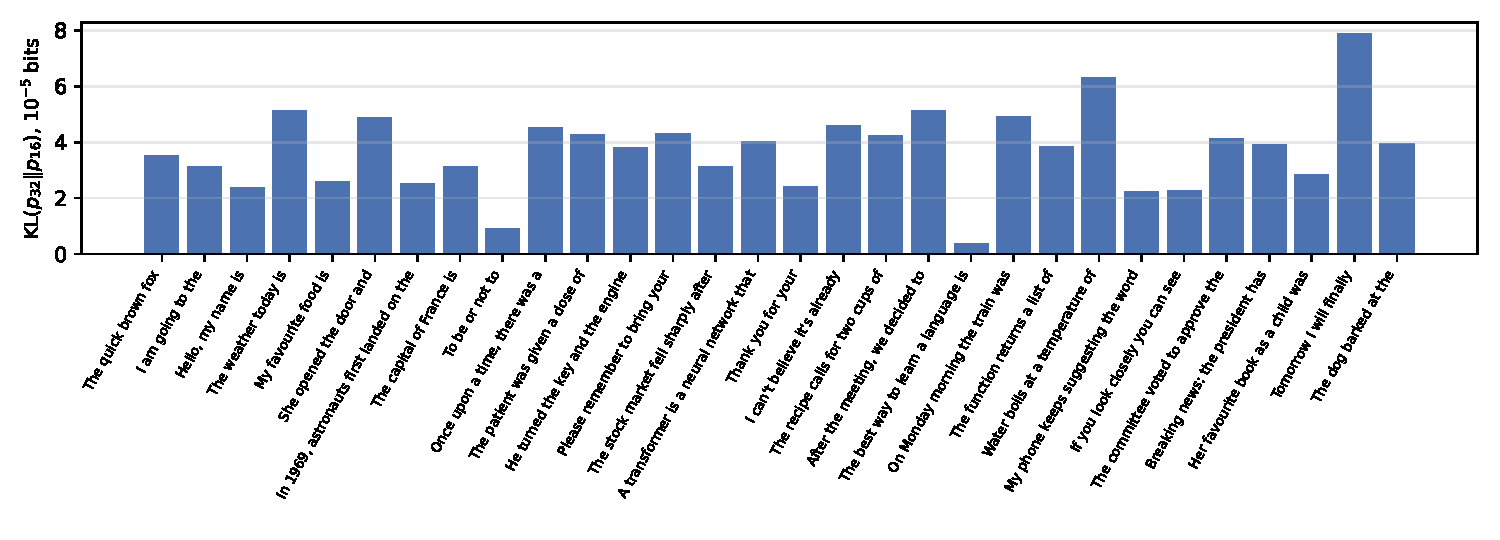
\includegraphics[width=\textwidth]{../figures/fig_fidelity.pdf}
\caption{KL divergence from the float32 model's next-token distribution to the float16-stored model's, per prompt. The largest value is $\FidKLMaxBits\times10^{-5}$ bits.}
\label{fig:fid}\end{figure}
The reference above shares the float16 weights with the app, so it tests the implementation, not the storage format. To measure the latter we run the NumPy forward pass over \FidPrompts\ prompts twice, once with the original float32 safetensors and once with the \texttt{TSW1} weights expanded to float32, and compare the full next-token distributions. The relative Frobenius error of the stored weights is $\FidWeightErrMedian\times10^{-4}$ (median over tensors, maximum $\FidWeightErrMax\times10^{-4}$). The top-1 token agrees on \FidTopOne/\FidPrompts\ prompts and the top-3 set on \FidTopThree/\FidPrompts; the mean KL divergence is $\FidKLMeanBits\times10^{-5}$ bits (Fig.~\ref{fig:fid}) and the largest change in any single probability is \FidMaxDp\ percentage points, on ``\FidWorstPrompt'' where ``\FidWorstToken'' moves from \FidWorstPthirtytwo\% to \FidWorstPsixteen\%. For an explanatory tool the format is lossless in every sense a user could notice, and it is consistent with the established practice of float16 inference \citep{micikevicius2018}.

\section{Performance}\label{sec:perf}
\subsection{Measurements}
The benchmark harness is part of the app. It is run either as a unit test or by launching the app with \texttt{-benchmark}, which writes \texttt{benchmark.json} into the app's documents folder on a physical phone. It records load time in three parts, forward latency for $T\in\{1,2,4,8,16,32,48\}$ tokens of a fixed paragraph (\RepeatsSim\ timed runs after three warm-ups, reporting the median and the 10th and 90th percentiles), physical memory footprint before load, after load and at peak, tokeniser throughput, and the device's thermal state.

\begin{table}[t]\centering\small
\begin{tabular}{lccccccc}\toprule
 & load & \multicolumn{5}{c}{traced forward pass, median (ms)} & $\Delta$footprint \\
\cmidrule(lr){3-7}
Device & (ms) & $T{=}1$ & 8 & 16 & 32 & 48 & (MB) \\\midrule
\DeviceRows
\bottomrule\end{tabular}
\caption{Load time, latency and memory. Debug configuration with \texttt{-O -Ounchecked}; thermal state \ThermalSim\ throughout. The footprint delta is the increase over the process baseline after loading the model.}
\label{tab:perf}\end{table}

\begin{figure}[t]\centering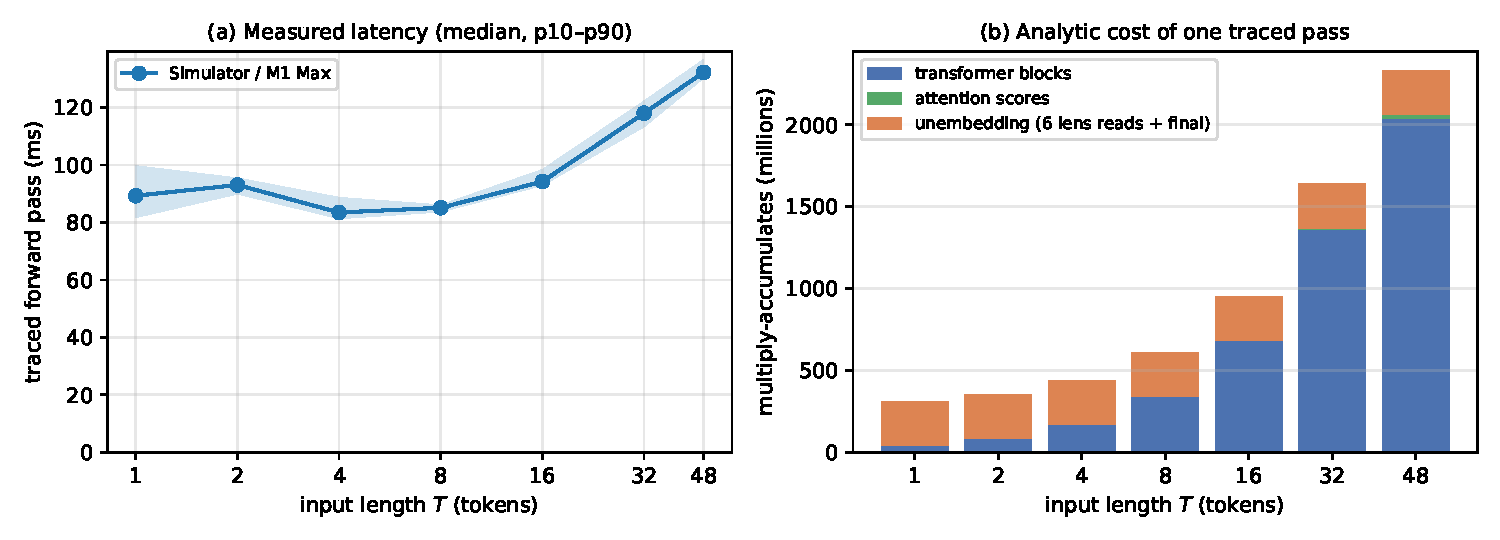
\includegraphics[width=\textwidth]{../figures/fig_latency.pdf}
\caption{(a) Measured latency of a traced pass against input length. (b) Multiply-accumulates for the same pass, split into the transformer blocks (linear in $T$), the attention score products (quadratic, negligible at these lengths) and the seven unembedding products (constant).}
\label{fig:lat}\end{figure}

Table~\ref{tab:perf} and Fig.~\ref{fig:lat}a give the numbers. \textbf{The measurements in this version were taken in the iOS Simulator on an Apple M1 Max (\OSVersionSim), which executes the same Accelerate code path on the host CPU. They characterise the engine, not a phone; iPhone measurements will replace them in a revision and the harness that produces them ships with the code.} Loading takes \LoadMsSim~ms: parsing the vocabulary JSON (\TokLoadMsSim~ms) and expanding float16 to float32 (\ExpandMsSim~ms) account for nearly all of it, and the memory map itself is free. The footprint rises by \FootprintDeltaMBSim~MB, which is the float32 copy of the weights (\WeightFpThirtyTwoMB~MB) plus the touched pages of the mapping; peak during inference is no higher, since activation buffers for 48 tokens are a few megabytes. Latency is flat at \LatShortMinSim--\LatShortMaxSim~ms for inputs of up to eight tokens and rises to \LatFortyEightSim~ms (p90 \LatFortyEightPninetySim~ms) at the 48-token cap, which keeps the interface interactive under a 250~ms input debounce. At 48 tokens the engine sustains about \GflopsFortyEightSim~GFLOP/s, well below what the hardware can do, which is the price of the unfused, trace-everything design.

\subsection{Why latency is flat for short inputs}
The shape of Fig.~\ref{fig:lat}a is explained by Fig.~\ref{fig:lat}b. The transformer blocks cost $\BlockMMACPerToken$~M multiply-accumulates per token. The unembedding $768\times\VocabSize$ product costs $\UnembedMMAC$~M, and a traced pass performs it seven times: once per layer for the logit lens and once at the output, for \UnembedTotalMMAC~M regardless of $T$. Table~\ref{tab:cost} tabulates the split. At one token the lens is \LensShareOne\% of the arithmetic; at 48 tokens it is \LensShareFortyEight\%. The attention score products are quadratic in $T$ but, with $d_h=64$ and $T\le48$, never exceed one percent. In other words, for the inputs a keyboard actually sees, the cost of \emph{explaining} the prediction exceeds the cost of \emph{making} it. A production keyboard model would have none of this overhead; ours has it by design.

\begin{table}[t]\centering\small
\begin{tabular}{cccccc}\toprule
$T$ & blocks (M MAC) & attention scores (M MAC) & unembedding $\times7$ (M MAC) & total & lens share \\\midrule
\CostRows
\bottomrule\end{tabular}
\caption{Analytic cost of one traced forward pass. Blocks: QKV, output projection and two MLP matmuls per layer. LayerNorm, bias, GELU and softmax are omitted (all $O(T d)$ or $O(T^2)$ and small).}
\label{tab:cost}\end{table}

\section{Discussion}\label{sec:discussion}
\paragraph{What a phone can show.} Everything, for a model of this size. The design question was never whether a phone could run an 82M-parameter model, which it plainly can, but whether it could run one in the transparent, unoptimised form that an explanation needs, on every keystroke, and still feel like a keyboard. The measurements say yes with margin: a traced pass is a tenth of a second, and the cost of the trace itself is a constant that a user never notices. The Weights screen answers the other half of the question: every weight is reachable, but only one tensor at a time, because the model has ten times more parameters than a 4K display has pixels. We think that observation is itself one of the more useful things the app teaches.

\paragraph{Design choices worth defending.} Recomputing the full sequence rather than caching is wasteful in a production engine and correct here, because the thing being shown is the algorithm, and a KV cache is an implementation detail that hides it. Expanding to float32 at load rather than running float16 kernels was chosen for simplicity and verifiability: it lets the engine use plain BLAS, lets the reference implementation be plain NumPy, and lets the oracle test be strict. The price is \WeightFpThirtyTwoMB~MB of memory and \ExpandMsSim~ms at launch. Keeping the Hugging Face weight layout means the converter is forty lines and the forward pass reads like the equations.

\paragraph{Limitations.} The timing results are from the simulator and are not yet a measurement of a phone; the harness for that exists and the gap will be closed in a revision. We report no learning outcomes: the Learn tab's effectiveness as pedagogy has not been evaluated with users, and we make no claim about it beyond describing what it does. The oracle test covers three prompts and two attention heads; the fidelity study covers thirty prompts. DistilGPT2 is a 2019 model trained on web text, and the app says so, but its suggestions can be odd or dated and the blocklist is a minimal courtesy rather than a safety system. Finally, the model is small enough to trace precisely because it is small; the approach does not scale to models whose attention tensors alone would exceed a phone's memory, and we do not suggest it should.

\section{Availability}\label{sec:avail}
Source (Swift, Python), the weight converter and NumPy reference, the benchmark harness and its raw results, the figure and macro scripts, and this manuscript are at \url{https://github.com/wonmor/OrchNeuralNetwork} under the MIT licence; the archived release is \doi{10.5281/zenodo.23142805} \citep{seong2026app}. Model weights are DistilGPT2 under Apache~2.0 \citep{sanh2019}. The app was submitted to the iOS App Store on 4~October 2026.

\section*{Author statement}
This work was conceived, designed and carried out by the author alone, without academic supervision, collaborators or institutional support. AI-assisted software tools were used in preparing the code and manuscript. The author takes full responsibility for all content and claims.

\begin{thebibliography}{99}
\bibitem[Apple(2024)]{apple2024} Apple. Apple Intelligence Foundation Language Models. arXiv:2407.21075 (2024).
\bibitem[Belrose et al.(2023)]{belrose2023} N.~Belrose, Z.~Furman, L.~Smith, D.~Halawi, I.~Ostrovsky, L.~McKinney, S.~Biderman, J.~Steinhardt. Eliciting latent predictions from transformers with the tuned lens. arXiv:2303.08112 (2023).
\bibitem[Bycroft(2023)]{bycroft2023} B.~Bycroft. LLM Visualization. \url{https://bbycroft.net/llm} (2023).
\bibitem[Cho et al.(2024)]{cho2024} A.~Cho, G.~C. Kim, A.~Karpekov, A.~Helbling, Z.~J. Wang, S.~Lee, B.~Hoover, D.~H. Chau. Transformer Explainer: Interactive learning of text-generative models. arXiv:2408.04619; IEEE VIS poster (2024).
\bibitem[Elhage et al.(2021)]{elhage2021} N.~Elhage, N.~Nanda, C.~Olsson, et al. A mathematical framework for transformer circuits. \emph{Transformer Circuits Thread} (2021).
\bibitem[Gerganov(2023)]{gerganov2023} G.~Gerganov. llama.cpp: LLM inference in C/C++. \url{https://github.com/ggerganov/llama.cpp} (2023).
\bibitem[Geva et al.(2021)]{geva2021} M.~Geva, R.~Schuster, J.~Berant, O.~Levy. Transformer feed-forward layers are key-value memories. \emph{EMNLP} (2021).
\bibitem[Hannun et al.(2023)]{hannun2023} A.~Hannun, J.~Digani, A.~Katharopoulos, R.~Collobert. MLX: Efficient and flexible machine learning on Apple silicon. \url{https://github.com/ml-explore/mlx} (2023).
\bibitem[Hard et al.(2018)]{hard2018} A.~Hard, K.~Rao, R.~Mathews, S.~Ramaswamy, F.~Beaufays, S.~Augenstein, H.~Eichner, C.~Kiddon, D.~Ramage. Federated learning for mobile keyboard prediction. arXiv:1811.03604 (2018).
\bibitem[Hendrycks and Gimpel(2016)]{hendrycks2016} D.~Hendrycks, K.~Gimpel. Gaussian error linear units (GELUs). arXiv:1606.08415 (2016).
\bibitem[Hoover et al.(2020)]{hoover2020} B.~Hoover, H.~Strobelt, S.~Gehrmann. exBERT: A visual analysis tool to explore learned representations in Transformer models. \emph{ACL System Demonstrations} (2020).
\bibitem[Micikevicius et al.(2018)]{micikevicius2018} P.~Micikevicius, S.~Narang, J.~Alben, et al. Mixed precision training. \emph{ICLR} (2018).
\bibitem[Nanda and Bloom(2022)]{nanda2022} N.~Nanda, J.~Bloom. TransformerLens. \url{https://github.com/TransformerLensOrg/TransformerLens} (2022).
\bibitem[nostalgebraist(2020)]{nostalgebraist2020} nostalgebraist. Interpreting GPT: the logit lens. \emph{LessWrong} (2020).
\bibitem[Radford et al.(2019)]{radford2019} A.~Radford, J.~Wu, R.~Child, D.~Luan, D.~Amodei, I.~Sutskever. Language models are unsupervised multitask learners. OpenAI technical report (2019).
\bibitem[Sanh et al.(2019)]{sanh2019} V.~Sanh, L.~Debut, J.~Chaumond, T.~Wolf. DistilBERT, a distilled version of BERT: smaller, faster, cheaper and lighter. arXiv:1910.01108 (2019). DistilGPT2 model card: \url{https://huggingface.co/distilgpt2}.
\bibitem[Sennrich et al.(2016)]{sennrich2016} R.~Sennrich, B.~Haddow, A.~Birch. Neural machine translation of rare words with subword units. \emph{ACL} (2016).
\bibitem[Seong(2026)]{seong2026app} W.~Seong. Orch Neural Network: an on-device GPT-2 visualiser for iOS (software). Zenodo (2026). \doi{10.5281/zenodo.23142805}
\bibitem[Vig(2019)]{vig2019} J.~Vig. A multiscale visualization of attention in the Transformer model. \emph{ACL System Demonstrations} (2019).
\end{thebibliography}
\end{document}
